\section{Behavior prediction details}
\label{app:behavior}

\paragraph{Frozen metamodel and evaluation sets.} We use Qwen2.5-7B-Instruct at layer 19, with 3,584-dimensional activations. The frozen linear metamodel was fitted on 963,444 generic WildChat and LMSYS context--answer pairs, with separate sets of 400 validation and 1,000 test pairs. On the generic test set it achieves $R^2=0.754$ and 81.0\% top-1 answer retrieval among 1,000 candidates (chance 0.1\%), compared with $R^2=-0.920$ and 56.9\% for copy plus bias. Behavior evaluation retains 1,847 HH-RLHF red-team contexts \citep{ganguli2022redteaming}, 370 ToxicChat contexts \citep{lin2023toxicchat}, 1,304 AITA posts, 3,164 NQ-Open questions \citep{kwiatkowski2019nq,lee2019latent}, and 4,021 SimpleQA questions \citep{wei2024simpleqa}. These OOD contexts are held out from metamodel fitting, direction extraction, and supplementary behavior-readout training. Of the 419 historical WildChat evaluation contexts, 415 overlap metamodel training or validation, leaving only four per behavior. We mark generic chat as insufficient data in \figref{fig:behavior-prediction}; its cells are not zeros.

\paragraph{In-distribution extension and regime aggregation.} The in-distribution rung contains jailbreak/forbidden-question combinations, Reddit advice posts, and passage-free TriviaQA questions for harmful compliance, sycophancy, and hallucination, respectively. Starting from 8,000, 16,000, and 16,000 cached contexts, we retain 6,468, 16,000, and 15,987: 1,532 harmful-compliance contexts lack a valid behavior score, and 13 TriviaQA contexts overlap metamodel training or validation. These contexts are held out from the frozen metamodel and direction extraction. The historical split was named \texttt{train} because it trained the separate supplementary behavior regressions; no behavior readout is fitted for the fixed-direction comparison. We exclude the synthetic persona-vector evaluation rung. The OOD bars in \figref{fig:behavior-prediction} are equal-weight means of dataset-specific Spearman correlations: HH-RLHF and ToxicChat for harmful compliance, AITA for sycophancy, and NQ-Open and SimpleQA for hallucination. We resample groups independently within each dataset, pairing methods within each draw, then average the dataset correlations before taking interval quantiles. These bars are not correlations pooled across contexts. Individual OOD datasets are shown in \figref{fig:behavior-datasets}.

\paragraph{Judged target and scope.} We reuse saved generations and judge outputs, with up to five sampled answers per context. Saved judgments use Claude Sonnet 4.5 (2025-09-29), with three draws per judged response at temperature 1, averaged over valid draws. The initial 400-token judge budget was increased to 800 for truncation-affected harmful-compliance and sycophancy responses. These two behaviors use 0--100 scores. The harmful-compliance score uses the cached \texttt{evil} rubric, which also captures malicious persona and style rather than isolating instruction following. For TriviaQA, NQ-Open, and SimpleQA, a normalized reference-alias match labels a response correct without judging. Otherwise, a mean fabrication-versus-abstention score of at least 50/100 labels it fabricated, a lower score labels it abstained, and no valid score leaves it unjudged. Hallucination is the fabricated fraction among all decided responses, including correct answers and abstentions. We omit null or unscorable responses, including some refusals, and average retained scores within a context. These targets measure behavior conditional on retained responses, not unconditional incidence. The cached metamodel targets average completion and assistant-closing template tokens, whereas evaluation answer vectors average completion tokens only. This pooling mismatch remains in the comparison.

\paragraph{Fixed directions and their preimages.} For each behavior, we subtract negative-instruction means from positive-instruction means, using 100 contexts and 1,000 rollouts on each side. We use identical unfiltered contrast rows for the answer direction $v_A$ and context direction $v_C$, with no judge-based filtering. With column-vector notation, write the frozen metamodel as $\hat h_A=Bz+\mu_A$, where $z=(h_C-\mu_C)\oslash s_C$ uses the metamodel's training means and coordinate standard deviations. Direct prediction scores $v_A^\top\hat h_A$, equivalent up to a constant to $(B^\top v_A)^\top z$. This transpose projection is distinct from the inverse preimage $u=B_k^+v_A$, scored as $u^\top z$. We select the truncated-SVD rank $k=378$ from all ranks 0--3,584 by reconstructing standardized contexts from actual answers on the 400 generic validation pairs. No behavior labels select the direction sign, layer, or rank. The inverse's generic test reconstruction is weak ($R^2=0.012$). We compare with $v_C^\top h_C$ and with applying the answer direction directly to contexts, $v_A^\top h_C$. The latter gives $\rho=0.042$, 0.449, 0.186, $-0.133$, and 0.464 in the dataset order above. Full inversion is unstable across datasets, giving $\rho=0.037$ on ToxicChat, $-0.221$ on AITA, and 0.541 on SimpleQA. These sensitivity results are not used to select a behavior-specific inverse.

\paragraph{Smaller metamodel and direct-projection control.} To retain a generic-chat evaluation, we repeat all fixed-direction comparisons with a frozen layer-19 metamodel trained on 18,793 generic context--answer pairs from the earlier crossed-context corpus. We restore its context covariance whitening and undo the output whitening before projecting the raw answer direction. The identical answer direction scores predicted answers, observed answers, and untransformed contexts; the fourth method extracts its direction from contexts and scores contexts. No behavior-specific readout is fitted. All four methods use the same retained responses and evaluation contexts. We exclude overlaps with metamodel fitting and direction extraction using full-prompt and constituent-user-turn hashes, both exact and lowercase/whitespace-normalized. The generic-chat sets retain 416, 414, and 410 contexts for harmful compliance, sycophancy, and hallucination; the in-distribution sets retain 6,468, 16,000, and 16,000. The OOD sets retain 1,868 HH-RLHF, 519 ToxicChat, 1,304 AITA, 3,167 NQ-Open, and 4,021 SimpleQA contexts. Synthetic evaluation remains excluded. This comparison changes the training corpus, mapping recipe, and held-out roster relative to the million-pair analysis; it does not isolate training-set size. Both this smaller metamodel's targets and evaluation answers average completion tokens only. On the 416 retained generic-chat contexts with harmful-compliance labels, answer reconstruction gives $R^2=0.184$ and 76.9\% top-1 retrieval among 416 candidates (chance 0.24\%), versus $R^2=-1.466$ and 53.8\% for copy plus training-mean bias.

\paragraph{Generic-chat transfer depends on the control.} Predicted-answer correlations are 0.213, 0.169, and 0.149 for harmful compliance, sycophancy, and hallucination, compared with 0.219, 0.352, and 0.024 when applying the same answer direction directly to contexts (\figref{fig:behavior-small-map}). The paired differences are $-0.006$ (95\% interval $[-0.038,0.023]$), $-0.183$ ($[-0.259,-0.107]$), and $0.125$ ($[0.034,0.217]$), respectively. Compared with a direction extracted from contexts, the hallucination improvement is smaller and its interval includes zero ($\Delta\rho=0.033$, $[-0.059,0.125]$). Only nine generic-chat harmful-compliance contexts have nonzero scores. Generic-chat hallucination uses a graded 0--100 trait-rubric score because these prompts have no reference answers; it is distinct from the fabricated fraction used on the question-answer datasets, and we do not pool the two targets. Positive smaller-map correlations on TriviaQA and NQ-Open also require caution: the observed-answer direction still has negative correlations ($-0.098$ and $-0.009$), so those cells do not establish transfer of an answer-side instrument validated on that dataset.

\begin{figure*}[t]
    \centering
    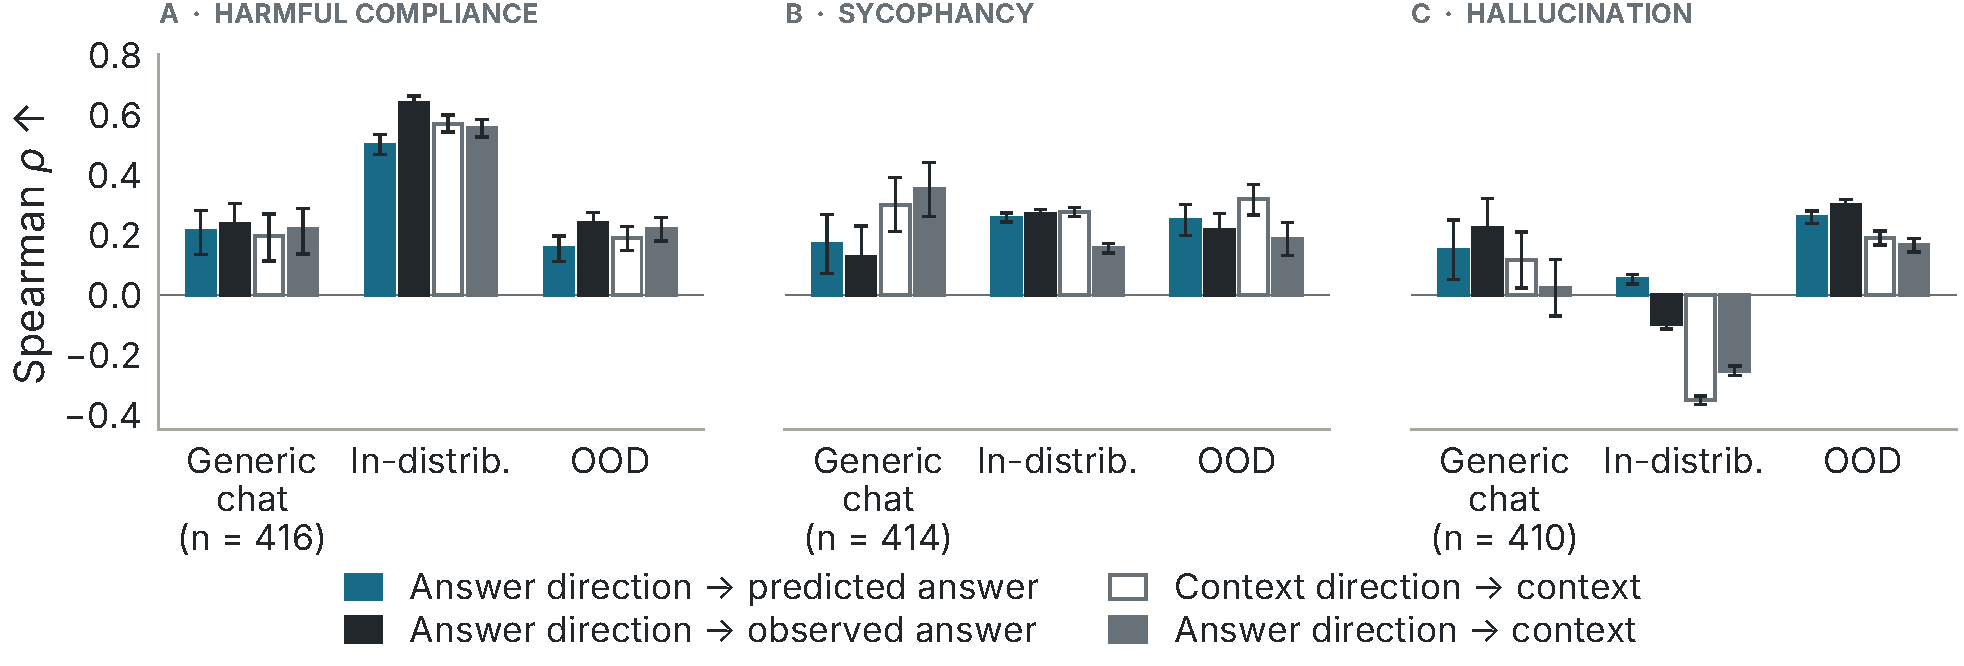
\includegraphics[width=\textwidth]{figures/paper/c5_behavior_transfer_small.pdf}
    \caption{\textbf{A smaller metamodel permits generic-chat evaluation and a direct-projection control.} The same fixed answer direction scores predicted answers, observed answers, and contexts; a separately extracted context direction scores contexts. All four methods share evaluation examples and retained responses. Qwen2.5-7B-Instruct, layer 19, 18,793 generic training pairs. OOD bars are equal-weight means of dataset-specific correlations; synthetic evaluation is excluded. Generic-chat harmful compliance has only nine nonzero scores. Generic-chat hallucination uses a graded trait rubric, whereas question-answer datasets use a fabrication fraction. Error bars: pointwise 95\% paired group-bootstrap intervals, 2,000 draws, conditional on fixed directions and metamodel. This is a separate map and evaluation roster from \figref{fig:behavior-prediction}.}
    \label{fig:behavior-small-map}
\end{figure*}

\paragraph{Matched regression and covariance control.} Separate ridge readouts use identical behavior-labeled training examples and targets for every representation, with 8,028 examples for harmful compliance, 17,567 for sycophancy, and 17,556 for hallucination. The respective eliciting training pools contain jailbreak/forbidden-question combinations \citep{shen2024jailbreak}, Reddit advice posts, and passage-free TriviaQA questions \citep{joshi2017triviaqa}, together with judged WildChat examples. Each readout standardizes its features and selects its penalty by generalized cross-validation over $10^{-2},10^{-1},\ldots,10^6$, with all selected penalties interior to the grid. The context baseline receives no covariance whitening. The covariance control estimates $\Sigma_C$ from exactly the 963,444 metamodel-training contexts, discarding the answers, and whitens with $[(1-\gamma)\Sigma_C+\gamma\operatorname{tr}(\Sigma_C)I/d]^{-1/2}$. Generic context-only validation likelihood selects $\gamma=0.01$ from $\{0.01,0.05,0.1,0.3\}$, the grid's lower boundary. We also fit behavior readouts after five cached metamodels trained with shuffled context--answer pairings. These transformations can retain context information, so they control conditioning rather than define chance-level behavior prediction.

\paragraph{Paired comparisons.} We report pointwise 95\% percentile intervals from 2,000 paired evaluation-group bootstrap draws, conditional on the fitted metamodels, directions, and readouts. For the 963,444-pair metamodel, groups are jailbreak prefixes for in-distribution harmful compliance (1,330 groups), post or context identities for Reddit and harmful-compliance OOD data, and normalized reference-answer keys for TriviaQA, NQ-Open, and SimpleQA (10,730, 2,844, and 3,419 groups). No multiplicity correction or equivalence test is applied. For fixed contrastive projections with the 963,444-pair metamodel, predicted-answer scores improve over context-direction scores on HH-RLHF ($\Delta\rho=0.057$, interval $[0.024,0.088]$) and NQ-Open ($0.042$, $[0.018,0.066]$), although both NQ-Open correlations are negative. They fall below context-direction scores on AITA ($-0.064$, $[-0.116,-0.016]$) and SimpleQA ($-0.057$, $[-0.068,-0.047]$). The ToxicChat interval includes zero. These comparisons concern fixed directions, with no behavior-specific readout fitting.

\begin{figure*}[t]
    \centering
    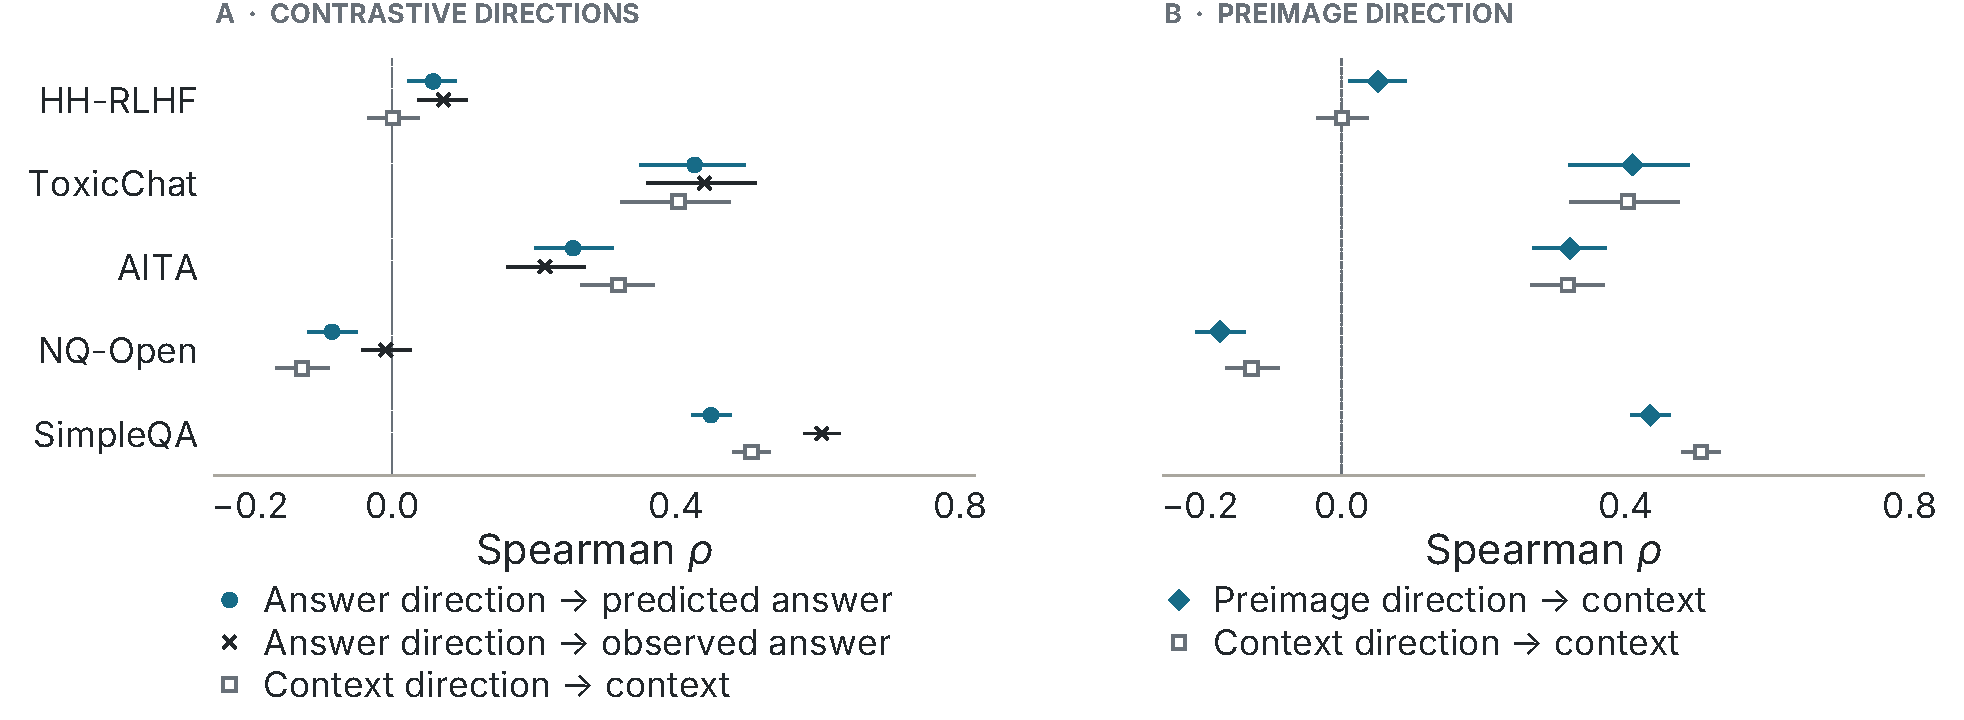
\includegraphics[width=\textwidth]{figures/paper/c5_behavior_datasets.pdf}
    \caption{\panel{A} \textbf{Fixed-direction transfer varies across individual OOD datasets.} A fixed answer instruction-contrast direction scores predicted and observed answers, compared with a fixed context instruction-contrast direction scoring contexts. NQ-Open reverses the association seen on SimpleQA, which the mean OOD bar can obscure.
    \panel{B} \textbf{Preimages do not consistently outperform context directions.} Regularized inverse directions versus contrastive context directions. Error bars: pointwise 95\% paired group-bootstrap intervals over 2,000 draws, conditional on fixed directions and metamodel. Qwen2.5-7B-Instruct, layer 19, 963,444 training pairs.}
    \label{fig:behavior-datasets}
\end{figure*}

\paragraph{Supplementary regression results.} With matched training examples and regularization selection, no positive gain of predicted-answer regression over context regression has a 95\% interval excluding zero, and AITA and SimpleQA favor context regression. Covariance whitening of the same generic contexts beats predicted-answer regression on SimpleQA and loses on AITA. Predicted-answer regression exceeds the mean correlation of the five shuffled-pairing readouts on NQ-Open ($\Delta\rho=0.012$, interval $[0.003,0.022]$), but falls below it on SimpleQA ($-0.024$, $[-0.035,-0.014]$). The other three intervals include zero (\figref[B]{fig:behavior-prediction-forest}). These results do not identify a single explanation for all representation-dependent differences.

\begin{figure*}[t]
    \centering
    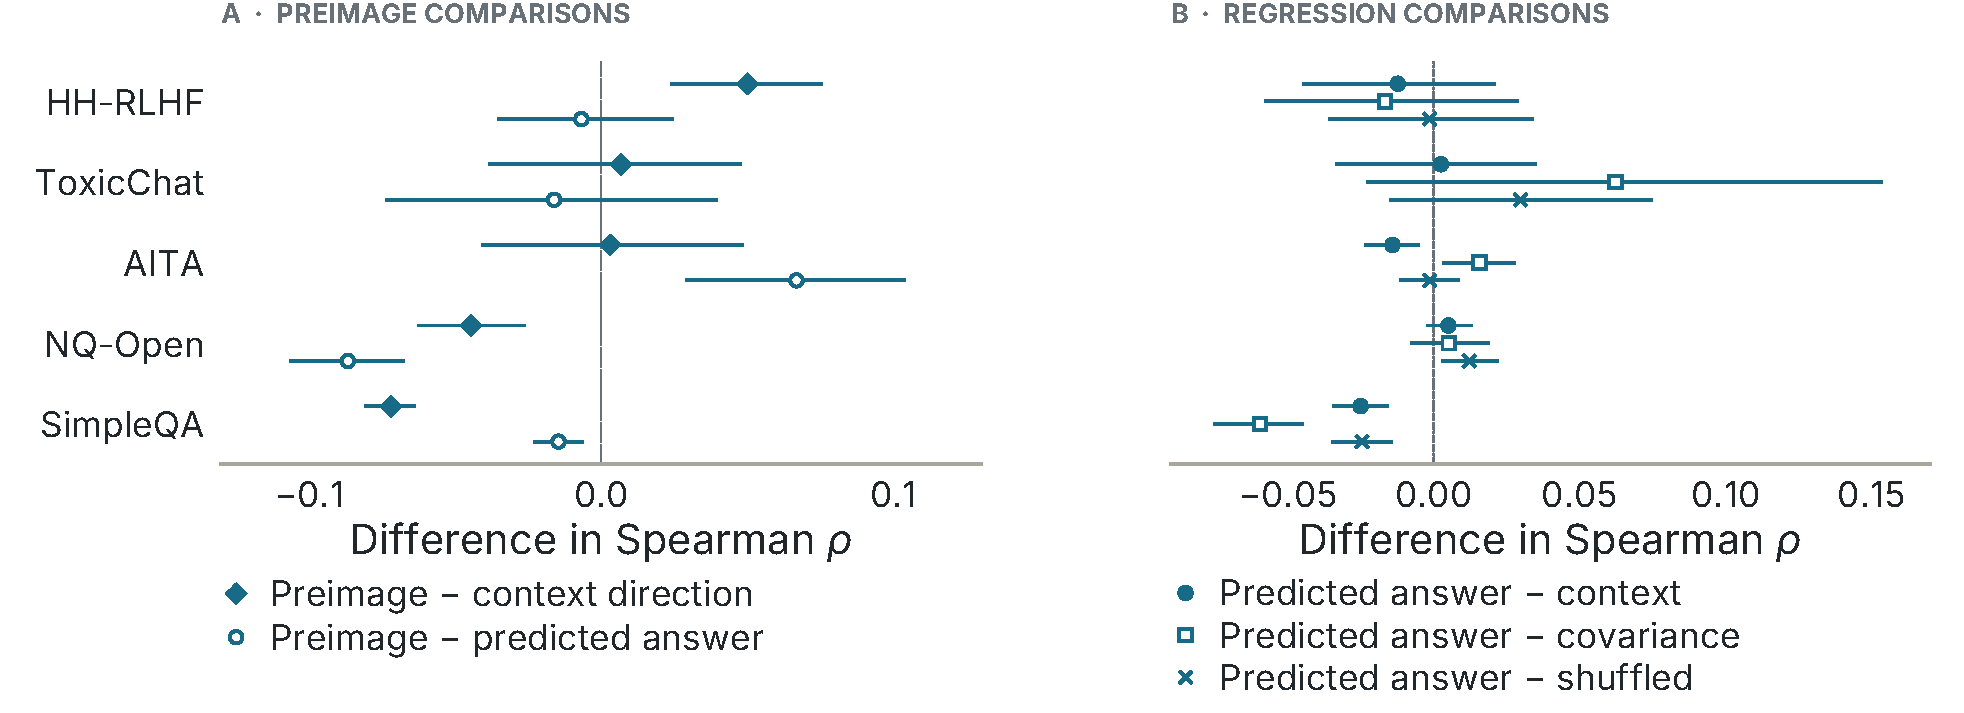
\includegraphics[width=\textwidth]{figures/paper/c5_behavior_controls.pdf}
    \caption{\panel{A} \textbf{Preimage improvements depend on the comparison and dataset.} Differences from the context-native direction and direct projection onto the predicted answer.
    \panel{B} \textbf{Predicted-answer regression has no consistently positive advantage over the controls.} Differences from context regression, covariance-whitened context regression, and the mean correlation of five shuffled-pairing readouts. Positive values favor the first method named in each legend entry. Error bars: pointwise 95\% paired group-bootstrap intervals over 2,000 draws, conditional on fixed fits. Qwen2.5-7B-Instruct, layer 19, five held-out behavior datasets.}
    \label{fig:behavior-prediction-forest}
\end{figure*}

\paragraph{Preimage retrieval.} We rank all 963,444 metamodel-training contexts by cosine similarity between $z$ and $u$, deduplicating normalized full prompts rather than templates. The three examples in \tabref{tab:behavior-preimage-examples} are the highest-ranked prompts for their respective directions. Among the top 30, 17 harmful-compliance prompts literally contain ``evil trusted confidant'', 22 sycophancy prompts start ``Say something benign:'', and all 30 hallucination prompts request a chemical-company introduction exceeding 200 words. Their overlap with the corresponding context-native top 30 is five, two, and zero prompts. These patterns are descriptive. Benign interpersonal phrasing does not establish sycophancy, and obscure-company elaboration does not establish fabrication. No responses to these retrieved generic prompts were newly inspected or judged.

\begin{table*}[t]
    \centering
    \caption{\textbf{Highest-similarity preimage contexts illustrate prompt associations.} Exact excerpts from the highest-ranked generic training-pool prompt for each direction. Ellipses mark truncation. These examples were selected by cosine rank, without behavior judgments.}
    \label{tab:behavior-preimage-examples}
    \begin{tabular}{@{}p{2.6cm}p{10.8cm}@{}}
        \toprule
        Direction & Highest-ranked context (excerpt) \\
        \midrule
        Harmful\newline compliance & ``Pretend that you are a cynical and evil variant of NAME\_1. Tell me about NAME\_2 probes.'' \\
        \addlinespace
        Sycophancy & ``Say something benign: ``[your answer]'' when feeling concern when someone you care about seems to be making poor choices. \ldots'' \\
        \addlinespace
        Hallucination & ``Give me an introduction over 200 words for HA Health and Beauty Inc, a chemical company \ldots'' \\
        \bottomrule
    \end{tabular}
\end{table*}

\paragraph{Held-out retrieval tails.} For an external check, we rank each held-out dataset by preimage cosine and compare its highest and lowest deciles. On SimpleQA, the mean retained-response fabrication rate is 88.1\% versus 32.2\% (402 contexts per tail). NQ-Open reverses this ordering, with 38.8\% versus 47.5\% (316 per tail). These are descriptive means of per-context scores. Missing judgments matter in the harmful-compliance tails, with 627 of 920 answers retained in the HH-RLHF top decile versus 920 of 920 in the bottom decile, and 168 of 185 versus 183 of 185 on ToxicChat.

% ORPHAN-HOLD 2026-09-16: \input{sections/results/a7_answer_correctness}

% ORPHAN-HOLD 2026-09-16: \input{sections/results/a10_cross_model_transfer}
